\documentclass[14pt,russian]{scrartcl}
\let\counterwithout\relax
\let\counterwithin\relax
\usepackage{lmodern}
\usepackage{float}
\usepackage{xcolor}
\usepackage{extsizes}
\usepackage{subfig}
\usepackage[export]{adjustbox}
\usepackage{tocvsec2} % возможность менять учитываемую глубину разделов в оглавлении
\usepackage[subfigure]{tocloft}

\usepackage{fancyvrb}
\usepackage{ulem,bm,mathrsfs,ifsym} %зачеркивания, особо жирный стиль и RSFS начертание
\usepackage{sectsty} % переопределение стилей подразделов
%%%%%%%%%%%%%%%%%%%%%%%

%%% Поля и разметка страницы %%%
\usepackage{pdflscape}                              % Для включения альбомных страниц
\usepackage{geometry}                               % Для последующего задания полей
\geometry{a4paper,tmargin=2cm,bmargin=2cm,lmargin=3cm,rmargin=1cm} % тоже самое, но лучше

%%% Математические пакеты %%%
\usepackage{amsthm,amsfonts,amsmath,amssymb,amscd}  % Математические дополнения от AMS
\usepackage{mathtools}                              % Добавляет окружение multlined
\usepackage[perpage]{footmisc}

%%%% Установки для размера шрифта 14 pt %%%%
%% Формирование переменных и констант для сравнения (один раз для всех подключаемых файлов)%%
%% должно располагаться до вызова пакета fontspec или polyglossia, потому что они сбивают его работу
%\newlength{\curtextsize}
%\newlength{\bigtextsize}
%\setlength{\bigtextsize}{13pt}
\KOMAoptions{fontsize=14pt}

\makeatletter
\def\showfontsize{\f@size{} point}
\makeatother

%\makeatletter
%\show\f@size                                       % неплохо для отслеживания, но вызывает стопорение процесса, если документ компилируется без команды  -interaction=nonstopmode 
%\setlength{\curtextsize}{\f@size pt}
%\makeatother

%шрифт times
\usepackage{tempora}

   %%% Решение проблемы копирования текста в буфер кракозябрами
%    \input glyphtounicode.tex
%    \input glyphtounicode-cmr.tex %from pdfx package
%    \pdfgentounicode=1
    \usepackage{cmap}                               % Улучшенный поиск русских слов в полученном pdf-файле
    \usepackage[T2A]{fontenc}                       % Поддержка русских букв
    \usepackage[utf8]{inputenc}                     % Кодировка utf8
    \usepackage[english, main=russian]{babel}            % Языки: русский, английский
%   \IfFileExists{pscyr.sty}{\usepackage{pscyr}}{}  % Красивые русские шрифты
%\renewcommand{\rmdefault}{ftm}
%%% Оформление абзацев %%%
\usepackage{indentfirst}                            % Красная строка
%\usepackage{eskdpz}

%%% Таблицы %%%
\usepackage{longtable}                              % Длинные таблицы
\usepackage{multirow,makecell,array}                % Улучшенное форматирование таблиц
\usepackage{booktabs}                               % Возможность оформления таблиц в классическом книжном стиле (при правильном использовании не противоречит ГОСТ)

%%% Общее форматирование
\usepackage{soulutf8}                               % Поддержка переносоустойчивых подчёркиваний и зачёркиваний
\usepackage{icomma}                                 % Запятая в десятичных дробях



%%% Изображения %%%
\usepackage{graphicx}                               % Подключаем пакет работы с графикой
\usepackage{wrapfig}

%%% Списки %%%
\usepackage{enumitem}

%%% Подписи %%%
\usepackage{caption}                                % Для управления подписями (рисунков и таблиц) % Может управлять номерами рисунков и таблиц с caption %Иногда может управлять заголовками в списках рисунков и таблиц
%% Использование:
%\begin{table}[h!]\ContinuedFloat - чтобы не переключать счетчик
%\captionsetup{labelformat=continued}% должен стоять до самого caption
%\caption{}
% либо ручками \caption*{Продолжение таблицы~\ref{...}.} :)

%%% Интервалы %%%

%%% Счётчики %%%
\usepackage[figure,table,section]{totalcount}               % Счётчик рисунков и таблиц
\DeclareTotalCounter{lstlisting}
\usepackage{totcount}                               % Пакет создания счётчиков на основе последнего номера подсчитываемого элемента (может требовать дважды компилировать документ)
\usepackage{totpages}                               % Счётчик страниц, совместимый с hyperref (ссылается на номер последней страницы). Желательно ставить последним пакетом в преамбуле

%%% Продвинутое управление групповыми ссылками (пока только формулами) %%%
%% Кодировки и шрифты %%%

%   \newfontfamily{\cyrillicfont}{Times New Roman}
%   \newfontfamily{\cyrillicfonttt}{CMU Typewriter Text}
	%\setmainfont{Times New Roman}
	%\newfontfamily\cyrillicfont{Times New Roman}
	%\setsansfont{Times New Roman}                    %% задаёт шрифт без засечек
%	\setmonofont{Liberation Mono}               %% задаёт моноширинный шрифт
 %   \IfFileExists{pscyr.sty}{\renewcommand{\rmdefault}{ftm}}{}
%%% Интервалы %%%
%linespread-реализация ближе к реализации полуторного интервала в ворде.
%setspace реализация заточена под шрифты 10, 11, 12pt, под остальные кегли хуже, но всё же ближе к типографской классике. 
\linespread{1.3}                    % Полуторный интервал (ГОСТ Р 7.0.11-2011, 5.3.6)
%\renewcommand{\@biblabel}[1]{#1}

%%% Гиперссылки %%%
\usepackage{hyperref}

%%% Выравнивание и переносы %%%
\sloppy                             % Избавляемся от переполнений
\clubpenalty=10000                  % Запрещаем разрыв страницы после первой строки абзаца
\widowpenalty=10000                 % Запрещаем разрыв страницы после последней строки абзаца

\makeatletter % малые заглавные, small caps shape
\let\@@scshape=\scshape
\renewcommand{\scshape}{%
  \ifnum\strcmp{\f@series}{bx}=\z@
    \usefont{T1}{cmr}{bx}{sc}%
  \else
    \ifnum\strcmp{\f@shape}{it}=\z@
      \fontshape{scsl}\selectfont
    \else
      \@@scshape
    \fi
  \fi}
\makeatother

%%% Подписи %%%
%\captionsetup{%
%singlelinecheck=off,                % Многострочные подписи, например у таблиц
%skip=2pt,                           % Вертикальная отбивка между подписью и содержимым рисунка или таблицы определяется ключом
%justification=centering,            % Центрирование подписей, заданных командой \caption
%}
%%%        Подключение пакетов                 %%%
\usepackage{ifthen}                 % добавляет ifthenelse
%%% Инициализирование переменных, не трогать!  %%%
\newcounter{intvl}
\newcounter{otstup}
\newcounter{contnumeq}
\newcounter{contnumfig}
\newcounter{contnumtab}
\newcounter{pgnum}
\newcounter{bibliosel}
\newcounter{chapstyle}
\newcounter{headingdelim}
\newcounter{headingalign}
\newcounter{headingsize}
\newcounter{tabcap}
\newcounter{tablaba}
\newcounter{tabtita}
%%%%%%%%%%%%%%%%%%%%%%%%%%%%%%%%%%%%%%%%%%%%%%%%%%

%%% Область упрощённого управления оформлением %%%

%% Интервал между заголовками и между заголовком и текстом
% Заголовки отделяют от текста сверху и снизу тремя интервалами (ГОСТ Р 7.0.11-2011, 5.3.5)
\setcounter{intvl}{3}               % Коэффициент кратности к размеру шрифта

%% Отступы у заголовков в тексте
\setcounter{otstup}{0}              % 0 --- без отступа; 1 --- абзацный отступ

%% Нумерация формул, таблиц и рисунков
\setcounter{contnumeq}{1}           % Нумерация формул: 0 --- пораздельно (во введении подряд, без номера раздела); 1 --- сквозная нумерация по всей диссертации
\setcounter{contnumfig}{1}          % Нумерация рисунков: 0 --- пораздельно (во введении подряд, без номера раздела); 1 --- сквозная нумерация по всей диссертации
\setcounter{contnumtab}{1}          % Нумерация таблиц: 0 --- пораздельно (во введении подряд, без номера раздела); 1 --- сквозная нумерация по всей диссертации

%% Оглавление
\setcounter{pgnum}{0}               % 0 --- номера страниц никак не обозначены; 1 --- Стр. над номерами страниц (дважды компилировать после изменения)

%% Библиография
\setcounter{bibliosel}{1}           % 0 --- встроенная реализация с загрузкой файла через движок bibtex8; 1 --- реализация пакетом biblatex через движок biber

%% Текст и форматирование заголовков
\setcounter{chapstyle}{1}           % 0 --- разделы только под номером; 1 --- разделы с названием "Глава" перед номером
\setcounter{headingdelim}{1}        % 0 --- номер отделен пропуском в 1em или \quad; 1 --- номера разделов и приложений отделены точкой с пробелом, подразделы пропуском без точки; 2 --- номера разделов, подразделов и приложений отделены точкой с пробелом.

%% Выравнивание заголовков в тексте
\setcounter{headingalign}{0}        % 0 --- по центру; 1 --- по левому краю

%% Размеры заголовков в тексте
\setcounter{headingsize}{0}         % 0 --- по ГОСТ, все всегда 14 пт; 1 --- пропорционально изменяющийся размер в зависимости от базового шрифта

%% Подпись таблиц
\setcounter{tabcap}{0}              % 0 --- по ГОСТ, номер таблицы и название разделены тире, выровнены по левому краю, при необходимости на нескольких строках; 1 --- подпись таблицы не по ГОСТ, на двух и более строках, дальнейшие настройки: 
%Выравнивание первой строки, с подписью и номером
\setcounter{tablaba}{2}             % 0 --- по левому краю; 1 --- по центру; 2 --- по правому краю
%Выравнивание строк с самим названием таблицы
\setcounter{tabtita}{1}             % 0 --- по левому краю; 1 --- по центру; 2 --- по правому краю

%%% Рисунки %%%
\DeclareCaptionLabelSeparator*{emdash}{~--- }             % (ГОСТ 2.105, 4.3.1)
\captionsetup[figure]{labelsep=emdash,font=onehalfspacing,position=bottom}

\captionsetup[lstlisting]{justification=raggedright, singlelinecheck=false}

%%% Таблицы %%%
\ifthenelse{\equal{\thetabcap}{0}}{%
    \newcommand{\tabcapalign}{\raggedright}  % по левому краю страницы или аналога parbox
}

\ifthenelse{\equal{\thetablaba}{0} \AND \equal{\thetabcap}{1}}{%
    \newcommand{\tabcapalign}{\raggedright}  % по левому краю страницы или аналога parbox
}

\ifthenelse{\equal{\thetablaba}{1} \AND \equal{\thetabcap}{1}}{%
    \newcommand{\tabcapalign}{\centering}    % по центру страницы или аналога parbox
}

\ifthenelse{\equal{\thetablaba}{2} \AND \equal{\thetabcap}{1}}{%
    \newcommand{\tabcapalign}{\raggedleft}   % по правому краю страницы или аналога parbox
}

\ifthenelse{\equal{\thetabtita}{0} \AND \equal{\thetabcap}{1}}{%
    \newcommand{\tabtitalign}{\raggedright}  % по левому краю страницы или аналога parbox
}

\ifthenelse{\equal{\thetabtita}{1} \AND \equal{\thetabcap}{1}}{%
    \newcommand{\tabtitalign}{\centering}    % по центру страницы или аналога parbox
}

\ifthenelse{\equal{\thetabtita}{2} \AND \equal{\thetabcap}{1}}{%
    \newcommand{\tabtitalign}{\raggedleft}   % по правому краю страницы или аналога parbox
}

\DeclareCaptionFormat{tablenocaption}{\tabcapalign #1\strut}        % Наименование таблицы отсутствует
\ifthenelse{\equal{\thetabcap}{0}}{%
    \DeclareCaptionFormat{tablecaption}{\tabcapalign #1#2#3}
    \captionsetup[table]{labelsep=emdash}                       % тире как разделитель идентификатора с номером от наименования
}{%
    \DeclareCaptionFormat{tablecaption}{\tabcapalign #1#2\par%  % Идентификатор таблицы на отдельной строке
        \tabtitalign{#3}}                                       % Наименование таблицы строкой ниже
    \captionsetup[table]{labelsep=space}                        % пробельный разделитель идентификатора с номером от наименования
}
\captionsetup[table]{format=tablecaption,singlelinecheck=off,font=onehalfspacing,position=top,skip=-5pt}  % многострочные наименования и прочее
\DeclareCaptionLabelFormat{continued}{Продолжение таблицы~#2}
\setlength{\belowcaptionskip}{.2cm}
\setlength{\intextsep}{0ex}

%%% Подписи подрисунков %%%
\renewcommand{\thesubfigure}{\asbuk{subfigure}}           % Буквенные номера подрисунков
\captionsetup[subfigure]{font={normalsize},               % Шрифт подписи названий подрисунков (не отличается от основного)
    labelformat=brace,                                    % Формат обозначения подрисунка
    justification=centering,                              % Выключка подписей (форматирование), один из вариантов            
}
%\DeclareCaptionFont{font12pt}{\fontsize{12pt}{13pt}\selectfont} % объявляем шрифт 12pt для использования в подписях, тут же надо интерлиньяж объявлять, если не наследуется
%\captionsetup[subfigure]{font={font12pt}}                 % Шрифт подписи названий подрисунков (всегда 12pt)

%%% Настройки гиперссылок %%%

\definecolor{linkcolor}{rgb}{0.0,0,0}
\definecolor{citecolor}{rgb}{0,0.0,0}
\definecolor{urlcolor}{rgb}{0,0,0}

\hypersetup{
    linktocpage=true,           % ссылки с номера страницы в оглавлении, списке таблиц и списке рисунков
%    linktoc=all,                % both the section and page part are links
%    pdfpagelabels=false,        % set PDF page labels (true|false)
    plainpages=true,           % Forces page anchors to be named by the Arabic form  of the page number, rather than the formatted form
    colorlinks,                 % ссылки отображаются раскрашенным текстом, а не раскрашенным прямоугольником, вокруг текста
    linkcolor={linkcolor},      % цвет ссылок типа ref, eqref и подобных
    citecolor={citecolor},      % цвет ссылок-цитат
    urlcolor={urlcolor},        % цвет гиперссылок
    pdflang={ru},
}
\urlstyle{same}
%%% Шаблон %%%
%\DeclareRobustCommand{\todo}{\textcolor{red}}       % решаем проблему превращения названия цвета в результате \MakeUppercase, http://tex.stackexchange.com/a/187930/79756 , \DeclareRobustCommand protects \todo from expanding inside \MakeUppercase
\setlength{\parindent}{2.5em}                       % Абзацный отступ. Должен быть одинаковым по всему тексту и равен пяти знакам (ГОСТ Р 7.0.11-2011, 5.3.7).

%%% Списки %%%
% Используем дефис для ненумерованных списков (ГОСТ 2.105-95, 4.1.7)
%\renewcommand{\labelitemi}{\normalfont\bfseries~{---}} 
\renewcommand{\labelitemi}{\bfseries~{---}} 
\setlist{nosep,%                                    % Единый стиль для всех списков (пакет enumitem), без дополнительных интервалов.
    labelindent=\parindent,leftmargin=*%            % Каждый пункт, подпункт и перечисление записывают с абзацного отступа (ГОСТ 2.105-95, 4.1.8)
}
%%%%%%%%%%%%%%%%%%%%%%
%\usepackage{xltxtra} % load xunicode

\usepackage{ragged2e}
\usepackage[explicit]{titlesec}
\usepackage{placeins}
\usepackage{xparse}

\usepackage{listingsutf8}
\usepackage{url} %пакеты расширений
\usepackage{algorithm, algorithmicx}
\usepackage[noend]{algpseudocode}
\usepackage{blkarray}
\usepackage{chngcntr}
\usepackage{tabularx}
\newcommand*\template[1]{\text{<}#1\text{>}}

  
\titleformat{name=\section,numberless}[block]{\normalfont\Large\centering}{}{0em}{#1}
\titleformat{\section}[block]{\normalfont\Large\bfseries\raggedright}{}{0em}{\thesection\hspace{0.25em}#1}
\titleformat{\subsection}[block]{\normalfont\Large\bfseries\raggedright}{}{0em}{\thesubsection\hspace{0.25em}#1}
\titleformat{\subsubsection}[block]{\normalfont\large\bfseries\raggedright}{}{0em}{\thesubsubsection\hspace{0.25em}#1}

\let\Algorithm\algorithm
\renewcommand\algorithm[1][]{\Algorithm[#1]\setstretch{1.5}}

\usepackage{relsize}
\usepackage{pifont}
\usepackage{calc}
\usepackage{suffix}
\usepackage{csquotes}
\DeclareQuoteStyle{russian}
    {\guillemotleft}{\guillemotright}[0.025em]
    {\quotedblbase}{\textquotedblleft}
\ExecuteQuoteOptions{style=russian}
\newcommand{\enq}[1]{\enquote{#1}}  
\newcommand{\eng}[1]{\begin{english}#1\end{english}}
% Подчиненные счетчики в окружениях http://old.kpfu.ru/journals/izv_vuz/arch/sample1251.tex
\newcounter{cTheorem} 
\newcounter{cDefinition}
\newcounter{cConsequent}
\newcounter{cExample}
\newcounter{cLemma}
\newcounter{cConjecture}
\newtheorem{Theorem}{Теорема}[cTheorem]
\newtheorem{Definition}{Определение}[cDefinition]
\newtheorem{Consequent}{Следствие}[cConsequent]
\newtheorem{Example}{Пример}[cExample]
\newtheorem{Lemma}{Лемма}[cLemma]
\newtheorem{Conjecture}{Гипотеза}[cConjecture]

\renewcommand{\theTheorem}{\arabic{Theorem}}
\renewcommand{\theDefinition}{\arabic{Definition}}
\renewcommand{\theConsequent}{\arabic{Consequent}}
\renewcommand{\theExample}{\arabic{Example}}
\renewcommand{\theLemma}{\arabic{Lemma}}
\renewcommand{\theConjecture}{\arabic{Conjecture}}
%\makeatletter
\NewDocumentCommand{\Newline}{}{\text{\\}}
\newcommand{\sequence}[2]{\ensuremath \left(#1,\ \dots,\ #2\right)}

\definecolor{mygreen}{rgb}{0,0.6,0}
\definecolor{mygray}{rgb}{0.5,0.5,0.5}
\definecolor{mymauve}{rgb}{0.58,0,0.82}
\renewcommand{\listalgorithmname}{Список алгоритмов}
\floatname{algorithm}{Листинг}
\renewcommand{\lstlistingname}{Листинг}
\renewcommand{\thealgorithm}{\arabic{algorithm}}

\newcommand{\refAlgo}[1]{(листинг \ref{#1})}
\newcommand{\refImage}[1]{(рисунок \ref{#1})}

\renewcommand{\theenumi}{\arabic{enumi}.}% Меняем везде перечисления на цифра.цифра	
\renewcommand{\labelenumi}{\arabic{enumi}.}% Меняем везде перечисления на цифра.цифра
\renewcommand{\theenumii}{\arabic{enumii}}% Меняем везде перечисления на цифра.цифра
\renewcommand{\labelenumii}{(\arabic{enumii})}% Меняем везде перечисления на цифра.цифра
\renewcommand{\theenumiii}{\roman{enumiii}}% Меняем везде перечисления на цифра.цифра
\renewcommand{\labelenumiii}{(\roman{enumiii})}% Меняем везде перечисления на цифра.цифра
%\newfontfamily\AnkaCoder[Path=src/fonts/]{AnkaCoder-r.ttf}
\renewcommand{\labelitemi}{---}
\renewcommand{\labelitemii}{---}

%\usepackage{courier}

\graphicspath{ {./img/} }

\lstdefinelanguage{Refal}{
  alsodigit = {.,<,>},
  morekeywords = [1]{$ENTRY},
  morekeywords = [2]{Go, Put, Get, Open, Close, Arg, Add, Sub, Mul, Div, Symb, Explode, Implode},
  %keyword4
  morekeywords = [3]{<,>},
  %keyword5
  morekeywords = [4]{e.,t.,s.},
  sensitive = true,
  morecomment = [l]{*},
  morecomment = [s]{/*}{*/},
  commentstyle = \color{mygreen},
  morestring = [b]",
  morestring = [b]',
  stringstyle = \color{purple}
}

\makeatletter
\def\p@subsection{}
\def\p@subsubsection{\thesection\,\thesubsection\,}
\makeatother
\newcommand{\prog}[1]{{\ttfamily\small#1}}
\lstset{ %
  backgroundcolor=\color{white},   % choose the background color; you must add \usepackage{color} or \usepackage{xcolor}
  basicstyle=\ttfamily\footnotesize, 
  %basicstyle=\footnotesize\AnkaCoder,        % the size of the fonts that are used for the code
  breakatwhitespace=false,         % sets if automatic breaks shoulbd only happen at whitespace
  breaklines=true,                 % sets automatic line breaking
  captionpos=top,                    % sets the caption-position to bottom
  commentstyle=\color{mygreen},    % comment style
  deletekeywords={...},            % if you want to delete keywords from the given language
  escapeinside={\%*}{*)},          % if you want to add LaTeX within your code
  extendedchars=true,              % lets you use non-ASCII characters; for 8-bits encodings only, does not work with UTF-8
  inputencoding=utf8,
  frame=single,                    % adds a frame around the code
  keepspaces=true,                 % keeps spaces in text, useful for keeping indentation of code (possibly needs columns=flexible)
  keywordstyle=\bf,       % keyword style
  language=Refal,                    % the language of the code
  morekeywords={<,>,$ENTRY,Go,Arg, Open, Close, e., s., t., Get, Put}, 
  							       % if you want to add more keywords to the set
  numbers=left,                    % where to put the line-numbers; possible values are (none, left, right)
  numbersep=5pt,                   % how far the line-numbers are from the code
  xleftmargin=25pt,
  xrightmargin=25pt,
  numberstyle=\small\color{black}, % the style that is used for the line-numbers
  rulecolor=\color{black},         % if not set, the frame-color may be changed on line-breaks within not-black text (e.g. comments (green here))
  showspaces=false,                % show spaces everywhere adding particular underscores; it overrides 'showstringspaces'
  showstringspaces=false,          % underline spaces within strings only
  showtabs=false,                  % show tabs within strings adding particular underscores
  stepnumber=1,                    % the step between two line-numbers. If it's 1, each line will be numbered
  stringstyle=\color{mymauve},     % string literal style
  tabsize=8,                       % sets default tabsize to 8 spaces
  title=\lstname                   % show the filename of files included with \lstinputlisting; also try caption instead of title
}
\newcommand{\anonsection}[1]{\cleardoublepage
\phantomsection
\addcontentsline{toc}{section}{\protect\numberline{}#1}
\section*{#1}\vspace*{2.5ex} % По госту положены 3 пустые строки после заголовка ненумеруемого раздела
}
\newcommand{\sectionbreak}{\clearpage}
\renewcommand{\sectionfont}{\normalsize} % Сбиваем стиль оглавления в стандартный
\renewcommand{\cftsecleader}{\cftdotfill{\cftdotsep}} % Точки в оглавлении напротив разделов

\renewcommand{\cftsecfont}{\normalfont\large} % Переключение на times в содержании
\renewcommand{\cftsubsecfont}{\normalfont\large} % Переключение на times в содержании

\usepackage{caption} 
%\captionsetup[table]{justification=raggedleft} 
%\captionsetup[figure]{justification=centering,labelsep=endash}
\usepackage{amsmath}    % \bar    (матрицы и проч. ...)
\usepackage{amsfonts}   % \mathbb (символ для множества действительных чисел и проч. ...)
\usepackage{mathtools}  % \abs, \norm
    \DeclarePairedDelimiter\abs{\lvert}{\rvert} % операция модуля
    \DeclarePairedDelimiter\norm{\lVert}{\rVert} % операция нормы
\DeclareTextCommandDefault{\textvisiblespace}{%
  \mbox{\kern.06em\vrule \@height.3ex}%
  \vbox{\hrule \@width.3em}%
  \hbox{\vrule \@height.3ex}}    
\newsavebox{\spacebox}
\begin{lrbox}{\spacebox}
\verb*! !
\end{lrbox}
\newcommand{\aspace}{\usebox{\spacebox}}


\title{Lab 02 report}
\author{Sergey}

\date{\today}

\begin{document}
\thispagestyle{empty}

\noindent \begin{minipage}{0.15\textwidth}
	
\includegraphics[width=\linewidth]{b_logo}
\end{minipage}
\noindent\begin{minipage}{0.85\textwidth}\centering
	\textbf{Министерство науки и высшего образования Российской Федерации}\\
	\textbf{Федеральное государственное бюджетное образовательное учреждение высшего образования}\\
	\textbf{«Московский государственный технический университет имени Н.Э.~Баумана}\\
	\textbf{(национальный исследовательский университет)»}\\
	\textbf{(МГТУ им. Н.Э.~Баумана)}
\end{minipage}

\noindent\rule{16cm}{3pt}
\newline\newline
\noindent ФАКУЛЬТЕТ $\underline{\text{«Информатика и системы управления»}}$ \newline\newline
\noindent КАФЕДРА $\underline{\text{«Программное обеспечение ЭВМ и информационные технологии»}}$\newline


\begin{center}
	\noindent\begin{minipage}{1.3\textwidth}\centering
	\Large\textbf{   ~~~ Лабораторная работа №5}\newline
	\textbf{по дисциплине "Анализ Алгоритмов"}\newline\newline\newline
	\end{minipage}
\end{center}

\noindent\textbf{Тема} $\underline{\text{Конвейерная обработка}}$\newline\newline
\noindent\textbf{Студент} $\underline{\text{Сабуров С. М.}}$\newline\newline
\noindent\textbf{Группа} $\underline{\text{ИУ7-53Б}}$\newline\newline
\noindent\textbf{Преподаватель} $\underline{\text{Волкова Л. Л.}}$\newline

\begin{center}
	\mbox{}
	\vfill
	Москва
\end{center}

\begin{center}
	\the\year ~г.
\end{center}
\clearpage

\renewcommand\contentsname{\hfill{\normalfont{СОДЕРЖАНИЕ}}\hfill}  %Оглавление
\tableofcontents
\newpage

\anonsection{Введение}

На сегодняшний день в мире существует огромное количество задач, решение которых
требует использования больших вычислительных мощностей, которые чаще всего
недоступны в современных вычислительных системах. В связи с этим, возрастают
требования к точности и к скорости решения таких задач. На помощь приходит создание параллельных вычислительных систем, в которых предусмотрена одновременная реализация ряда вычислительных процессов, связанных с решением одной задачи, что на сегодняшний день является одним из основных способов ускорения вычислений. При таком подходе увеличение производительности достигается путем параллельного выполнения частей более сложной задачи.



Целью данной работы является получение навыка реализации метода конвейерных
вычислений.



Для достижения поставленной цели необходимо выполнить следующие задачи:
\begin{itemize}
    \item описать методы обработки данных и  сопоставить их с  методами конвейера.
    \item привести схемы конвейера.
    \item реализовать конвейерную систему, описать данную реализацию.
    \item сравнить  временные характеристики экспериментально.
    \item на основании проделанной работы сделать выводы.
\end{itemize}

\section{Аналитическая часть}






В данном разделе будет описана идея конвейерной обработки.

\subsection{Конвейерная обработка}
Конвейеризация – это техника, в результате которой задача или команда разбивается на некоторое число подзадач, которые выполняются
последовательно. Каждая подкоманда выполняется на своем логическом
устройстве. Все логические устройства (ступени) соединяются последовательно и работают одновременно. Множество ступеней называется
конвейером. Выигрыш во времени достигается при выполнении нескольких
задач за счет параллельной работы ступеней, вовлекая на каждом такте
новую задачу или команду.


\subsection{Область применения}
	Для данной лабораторной работы был разработан алгоритм шифрования строк, состоящий из трех этапов:
	
	\begin{itemize}
    \item шифрование методом цезаря.
    \item алгоритм, в котором к символу строки прибавляется сумма порядковых номеров символов всей строки из таблицы ASCII и порядковый номер  символа в строке(индекс).
    \item алгоритм перестановки двух соседних символов.
\end{itemize} . \subsection{Вывод}

В данном разделе была поставлена задача реализации  конвейерных вычислений . Была описана идея конвейеризации. 

\begin{itemize}
	\item Входные данные :количество слов в тексте.
	\item Выходные данные : на выходе имеем зашифрованный текст.
	\item Ограничения, в рамках которых будет работать программа : количество слов должно быть задано натуральным числом.
	\item Функциональные требования : функции, представленные на листингах 1 - 3 должны корректно шифровать исходный текст.
	\item Требования к программному обеспечению : к программе предъявляется ряд требований:
			\begin{itemize}
			    \item на вход подается количество слов, размер слова задан константой, программа сама генерирует слова, необязательно осмысленные;
			    \item на выходе - результат конвейеронго шифрования.
			\end{itemize}
\end{itemize}

\section{Конструкторская часть}
В данном разделе будут приведены схемы  алгоритмов, описание структур данных, способы тестирования и классы эквивалентности.

\subsection{Разработка алгоритмов}

На рисунках \ref{img:classic}-\ref{img:parallel} приведены схемы работы конвейера и его составных частей.

\subsection{Описание структур данных}
Конвейер был преставлен в виде очереди. Текст хранился в виде массива строк.

\subsection{Способы тестирования и классы эквивалентности}
Была выбрана методика тестирования черным ящиком. 
Классы эквивалентности:
\begin{itemize}
	\item Текст состоит из 1 строки.
	\item Текст состоит из 0 строк.
	\item Текст состоит из n строк, n - натуральное число.
	\item Задано количество строк - не натуральное число.
\end{itemize}
\subsection{Вывод}

На основе теоретических данных, полученных из аналитического раздела, были построены схемы требуемых алгоритмов, описаны стртуктуры данных, выделены способы тестирования и классы эквивалентности.

\begin{figure}
    \centering
    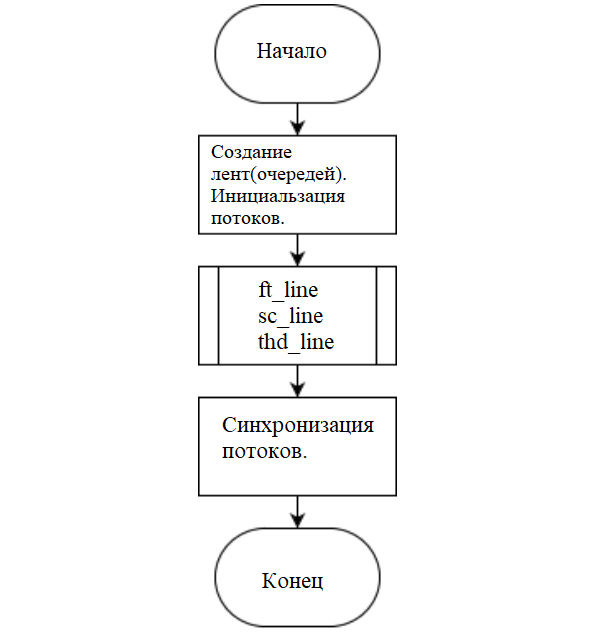
\includegraphics[scale=0.75]{shema_1.png}
    \caption{Схема запуска конвейера.}
    \label{img:classic}
\end{figure}

\begin{figure}
    \centering
    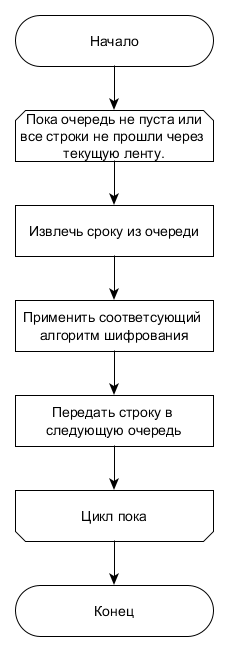
\includegraphics[scale=0.75]{schema_2.png}
    \caption{Схема работы ленты конвейера}
    \label{img:parallel}
\end{figure}



\section{Технологическая часть}

В данном разделе приведены требования к программному обеспечению, средства реализации и листинги кода.



\subsection{Средства реализации}


Для реализации программ был выбран язык программирования C++ [1]. Данный язык был выбран потому, что в нем присутствует инструментарий для замера процессорного времени и тестирования.


\begin{lstlisting}[caption=Первый алгоритм шифрование: Метод цезаря, label=list:canon, language={}]
string encrypt_1(string s)
{
	
	for (int i = 0; i < s.length(); i++)
	{
		try
		{

			if (s[i] == 'z')
			{
				s[i] = 'a';
			}
			else if (s[i] == 'Z')
				s[i] = 'A';
			else
				s[i] = s[i] + 1;
		}
		catch(...)
		{
			cout << "ENCRYPT 1" << s << endl;
		}

	}
	return s;
}\end{lstlisting}
\begin{lstlisting}[caption=Второй алгоритм шифрование: Пользовательский метод, описанный в аналитическом разделе, label=list:canon, language={}]
string encrypt_2(string s)
{
	

	int sum = 0;
	for (int i = 0; i < s.length(); i++)
	{
		sum += s[i];
	}
	for (int i = 0; i < s.length(); i++)
	{
		try
		{

			if (s[i] >= 'a' && s[i] <= 'z')
			{
				s[i] = (s[i] + sum + i) % ('z' - 'a') + 'a';

			}
			else if (s[i] >= 'A' && s[i] <= 'Z')
			{
				s[i] = (s[i] + sum + i) % ('Z' - 'A') + 'A';
			}
		}
		catch (...)
		{
			cout << "ENCRYPT 2 " << s << endl;
		}
		
	}
	return s;
}
\end{lstlisting}
\begin{lstlisting}[caption=Третий алгоритм шифрование: Перестановка соседних символов, label=list:canon, language={}]
string encrypt_3(string s)
{
	if (s.length() > 0)
	{

		for (int i = 0; i < s.length() - 1; i+= 2)
		{
			try
			{
				char tmp = s[i];
				s[i] = s[i + 1];
				s[i + 1] = tmp;
			}
			catch (...)
			{
				cout << "ENCRYPT 3" << s << endl;
			}
		}
	}
	return s;
}
\end{lstlisting}
\begin{lstlisting}[caption=Реализация первой ленты конвейера, label=list:canon, language={}]
void ft_line()
{

	int num = 0;

	while (true) {
		if (num == n)
			break;
		m1.lock();
		if (q1.empty()) {
			m1.unlock();
			continue;
		}
		string cur_str  = q1.front();
		q1.pop();

		m1.unlock();
		string new_str = encrypt_1(cur_str);
		m2.lock();
		
		q2.push(new_str);
		m2.unlock();
		num++;
	}


}

\end{lstlisting}

\begin{lstlisting}[caption=Реализация второй ленты конвейера, label=list:canon, language={}]
void sc_line()
{
	int num = 0;
	while (true) {
		if (num == n)
			break;
		m2.lock(); // wait in queue
		if (q2.empty()) {
			m2.unlock();
			continue;
		}
		string cur_str = q2.front();
		q2.pop();

		m2.unlock();
		string new_str = encrypt_2(cur_str);
		m3.lock();
		
		q3.push(new_str);
		m3.unlock();
		num++;
	}
}
\end{lstlisting}

\begin{lstlisting}[caption=Реализация третий ленты конвейера, label=list:canon, language={}]
void thd_line()
{
	int num = 0;
	while (true) {
		if (num == n)
			break;
		m3.lock(); // wait in queue
		if (q3.empty()) {
			m3.unlock();
			continue;
		}
		string cur_str = q3.front();
		q3.pop();

		m3.unlock();
		string new_str = encrypt_3(cur_str);
		resm.lock();
		
		q_final.push(new_str);
		resm.unlock();
		num++;
	}
}
\end{lstlisting}



\subsection{Тестирование функций}

В таблице \ref{tab:tests} приведены модульные тесты для функций шифрования текста. Все тесты были пройдены успешно. \\

\begin{table}[hb]
    \caption{\centering Тестирование функций шифрования строки}
    \centering
    \begin{tabular}{|c|c|}
    \hline
    Исходная строка & Ожидаемый результат \\ \hline
    %$\begin{pword}
        Hello & iDrqv \\ \hline
        123 & 324 \\ \hline
        H & V \\ \hline
        hello world & idrqv nnmrf \\ \hline
        <Пустая строка> & Шифрование невозможно \\ \hline
    %\end{pword}$
    \end{tabular}
    \label{tab:tests}
    \end{table}

\subsection{Вывод}

Были разработаны реализации алгоритмов шифрования и конвейеризации соотвественно. Также были протестированы реализации алгоритмов шифрования.

\section{Исследовательская часть}
В данном разделе будут приведены результаты исследовательской деятельности - замеры процессорного времени работы алгоритмов и тестирование алгоритмов.

\subsection{Технические характеристики}

Технические характеристики электронно-вычислительнй машины, на которой выполнялось тестирование:

\begin{itemize}
    \item операционная система: Windows 10 64-bit;
    \item оперативная память: 8 гигабайт ;
    \item процессор: Intel i5 7th gen.
\end{itemize}


Тестирование проводилось на ноутбуке, включенном в сеть электропитания. Во время тестирования ноутбук был нагружен только встроенными приложениями окружения рабочего стола, окружением рабочего стола, а также непосредственно системой тестирования.

\subsection{Время выполнения алгоритмов}

Был проведен замер времени работы каждого из алгоритмов с помощью функции std::chrono::system clock::now. Эта функция замеряет процессорное время выполнения функции и усредняет его (проводится 10 замеров). В таблице \ref{tab:time_best} содержатся результаты исследований. В таблице \ref{tab:time_log} содержится лог программы.

На рисунке \ref{img:plot_best} демонстрируется зависимость времени выполнения последовательного и конвейерного алгоритмов от количества строк. \\

\begin{table}[ht]
    \caption{\centering Время выполнения реализаций алгоритмов (в секундах) при количестве символов в строке 5000.}
    \centering
    \begin{tabular}{|c|c|c|c|}
    \hline
    Кол-во строк & К      & П     \\ \hline
    100    & 0.246199 & 0.555688 \\ \hline
    500    & 1.15154 & 2.75488  \\ \hline
    1000    & 2.36791  & 5.77721  \\ \hline
    2500    & 5.80938  & 14.0969  \\ \hline
    5000    & 11.7832  & 28.8174  \\ \hline
    10000    & 24.1511  & 55.4429  \\ \hline
 
    \end{tabular}
    \label{tab:time_best}
\end{table}


\begin{table}[ht]
    \caption{\centering Лог программы при количестве строк 5.}
    \centering
    \begin{tabular}{|c|c|c|c|c|}
    \hline
    Линия № & Строка №     & Время начала (мс)  & Время конца (мс)  \\ \hline
    1    & 0 & 7.227e+06   & 7.2795e+06 \\ \hline
    2    & 0 & 1.3869e+07   & 1.39594e+07\\ \hline
    1    & 1 & 1.39611e+07   & 1.39689e+07\\ \hline
    3    & 0 & 1.8941e+07 & 1.89564e+07 \\ \hline
    1    & 2 & 2.03209e+07  & 2.0327e+07\\ \hline
    2    & 1 & 2.03243e+07  & 2.03323e+07\\ \hline
    1    & 3 & 2.32028e+07  & 2.32085e+07\\ \hline
    2    & 2 & 2.6129e+07  & 2.61349e+07\\ \hline
    3    & 1 & 2.66033e+07  & 2.66153e+07\\ \hline
    1    & 4 & 2.76257e+07  & 2.7632e+07\\ \hline
    2    & 3 & 3.13649e+07  &3.13702e+07\\ \hline
    3    & 2 & 3.75349e+07  & 3.21479e+07\\ \hline
    2    & 4 & 3.75349e+07  & 3.75402e+07\\ \hline
    3    & 3 &3.75711e+07  & 3.75798e+07\\ \hline
    3    & 4 & 4.19849e+07  & 4.19913e+07\\ \hline
    \end{tabular}
    \label{tab:time_log}
\end{table}

\begin{figure}
    \centering
    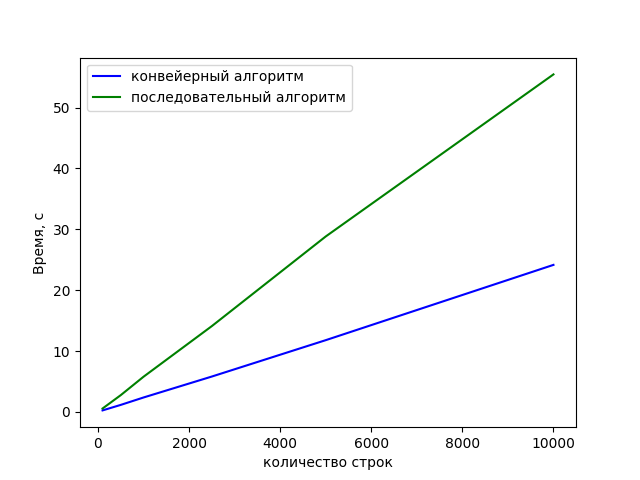
\includegraphics[scale=0.85]{plot.png}
    \caption{Зависимость времени выполнения алгоритмов от количества строк}
    \label{img:plot_best}
\end{figure}

\subsection{Вывод}

В данном разделе было произведено сравнение количества затраченного времени вышеизложенных алгоритмов.
Конвейерная реализация значительно выигрывает
по времени в сравнении с  линейной реализации. Как видно из рисунка 4, линейная
реализация примерно в 2 раза медленнее параллельной при 10000 строках.


\anonsection{Заключение}


В ходе выполнения работы была достигнута цель выполнены все поставленные задачи:

\begin{itemize}
    \item описать методы обработки данных и  сопоставить их с  методами конвейера.
    \item привести схемы конвейера.
    \item Реализовать конвейерную систему, описать данную реализацию
    \item сравнить  временные характеристики экспериментально;
    \item на основании проделанной работы сделать выводы.
\end{itemize}

Экспериментально были установлены различия в производительности алгоритмов. Конвейерный алгоритм  имеет большую эффективность, нежели линейный алгоритм. 
\anonsection{Список литература}

	\begin{enumerate}

		\item Т. Кормен, Ч. Лейзерсон, Р. Ривест, К. Штайн. Алгоритмы. Построение и анализ. Издательский дом ``Вильямс'', 2011. 282 - 315.
		\item Б. Страуструп. Язык программирования С++ . Addison-Wesley, 2000. 257 - 279.
		\item Конвейерные вычисления [Электронный ресурс].Режим доступа: http://www.myshared.ru/slide/674082 
		\item Корнеев В.В. Параллельные вычислительные системы. М., 1999. 320 с.
		\item Р. Седжвик. Фундаментальные алгоритмы С++. Diasoft, 2001. 567 - 597.

	\end{enumerate}

\end{document}
